\documentclass[12pt, oneside]{article}
\usepackage[letterpaper, margin=1in, headsep=0.5in]{geometry}
\usepackage[english]{babel}
\usepackage[utf8]{inputenc}
\usepackage{amsmath}
\usepackage{amsfonts}
\usepackage{amssymb}
\usepackage{tikz}
\usetikzlibrary{quotes, angles}
\usepackage{graphicx}
%\usepackage{pgfplots}
%\pgfplotsset{width=10cm,compat=1.9}
%\usepgfplotslibrary{statistics}
%\usepackage{pgfplotstable}
%\usepackage{tkz-fct}
%\usepackage{venndiagram}

\usepackage{fancyhdr}
\pagestyle{fancy}
\fancyhf{}
\rhead{\thepage \\Name: \hspace{1.5in}.\\}
\lhead{BECA / Dr. Huson / Geometry 10th Grade\\* Learning trajectory: Constructions}

\renewcommand{\headrulewidth}{0pt}

\begin{document}
\subsubsection*{Classical constructions}
\begin{enumerate}
  \item Elementary, single constuctions
  \begin{enumerate}
    \item Equilateral Triangle
    \item Duplicate a line segment
    \item Perpendicular (bisector, through a point on/off the line)
    \item Bisect an angle
    \item Duplicate an angle
    \end{enumerate}
  \item Triangle centers (perpendicular, bisectors, altitudes, medians)
  %\item Hexagon and square inscribed in a circle
  %\item Triangle midline
  \end{enumerate}

\begin{enumerate}
\subsubsection*{Equilateral triangle}
  \item Construct an equilateral triangle having one side on $\overrightarrow{T}$ with each leg congruent to $\overline{AB}$.
  [Leave all construction marks.]\\
    \vspace{5cm}
    \begin{center}
    \begin{tikzpicture}
      \draw [-, thick] (0,3)--(3,0);
      \draw [->, thick] (4,-3)--(11,-3);
      \draw [fill] (4,-3) circle [radius=0.05] node[above left]{$T$};
      \draw [fill] (0,3) circle [radius=0.05] node[above left]{$A$};
      %\node at (8.5,-0.4){$l$};
      \draw [fill] (3,0) circle [radius=0.05] node[below right]{$B$};
    \end{tikzpicture}
    \end{center}
    \vspace{2cm}

\newpage
\subsubsection*{Perpendicular (bisector, through a point on/off the line)}
  \item Construct a perpendicular bisector the given line segment $\overline{AB}$. Label the midpoint of $\overline{AB}$ as $M$.  [Leave all construction marks.]\\
    \vspace{2cm}
    \begin{center}
    \begin{tikzpicture}
      \draw [-, thick] (0,3)--(3,0);
      \draw [fill] (0,3) circle [radius=0.05] node[above left]{$A$};
      %\node at (8.5,-0.4){$l$};
      \draw [fill] (3,0) circle [radius=0.05] node[below right]{$B$};
    \end{tikzpicture}
    \end{center}
    \vspace{2cm}

\subsubsection*{Angle bisector}
  \item Construct an angle bisector the given angle $A$.  [Leave all construction marks.]\\
      \vspace{2cm}
      \begin{center}
      \begin{tikzpicture}
        \draw [<->, thick] (-2,5)--(0,0)--(7,0);
        \draw [fill] (0,0) circle [radius=0.05] node[below]{$A$};
        %\draw [fill] (7,0) circle [radius=0.05] node[below]{$N$};
      \end{tikzpicture}
      \end{center}

\newpage
\subsubsection*{Triangle centers}

  \item Construct a perpendicular to $\overline{AB}$ through $C$.\\
    %\hspace{1cm} Given the line  $l$ and point $P$.
    \vspace{1cm}
    \begin{center}
    \begin{tikzpicture}
      \draw [<->, thick] (0,0)--(11,0)--(7,3)--cycle;
      \draw [fill] (0,0) circle [radius=0.05] node[left]{$A$};
      \draw [fill] (11,0) circle [radius=0.05] node[right]{$B$};
      \draw [fill] (7,3) circle [radius=0.05] node[above right]{$C$};
    \end{tikzpicture}
    \end{center}
    \vspace{4cm}

  \item Construct the midpoint $M$ of $\overline{AC}$ by using the perpendicular bisector construction. Draw $\overline{BM}$, a \emph{median} of $\triangle ABC$.\\
  Spicy: Construct the other two medians, and hence, the centroid.
    \vspace{1cm}
    \begin{center}
    \begin{tikzpicture}
      \draw [<->, thick] (0,0)--(6.5,0)--(6,4)--cycle;
      \draw [fill] (0,0) circle [radius=0.05] node[left]{$A$};
      \draw [fill] (6.5,0) circle [radius=0.05] node[right]{$B$};
      \draw [fill] (6,4) circle [radius=0.05] node[above right]{$C$};
    \end{tikzpicture}
  \end{center} \vspace{1.5cm}

\newpage
    \item In the circle below, $\overline{AB}$ is a chord. Using a compass and straightedge, construct a perpendicular bisector of $\overline{AB}$, and hence, a diameter of the circle. [Leave all construction marks.]\\[4cm]
    \begin{center}
    \begin{tikzpicture}[scale=.635]
      %\draw [help lines] (-4,-4) grid (4,4);
      \draw [thick, -] (-5,0) node[left]{$A$} -- (0,5) node[above]{$B$};
      %\draw [thick, ->] (0,-2.2)--(0,10.4) node [left] {$y$};
      \draw (0,0) circle [radius=5]; %node[below]{$C$};
      %\draw [fill] (0,0) circle [radius=0.05];
    \end{tikzpicture}
    \end{center}

\newpage
  \item Spicy: Given $\angle ABC$, construct duplicate $\angle CDE$. (Leave all construction marks.)
    \begin{center}
    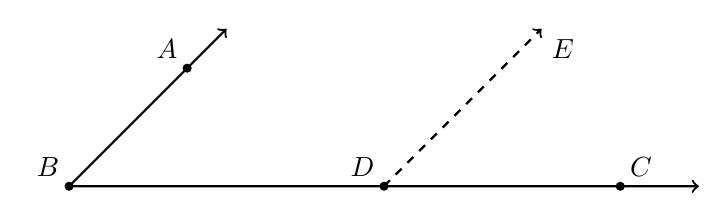
\begin{tikzpicture}
      \draw [<->, thick] (2,2)--(0,0)--(8,0);
      \draw [->, thick, dashed] (4,0)--(6,2) node[below right]{$E$};
      \draw [fill] (1.5,1.5) circle [radius=0.05] node[above left]{$A$};
      \draw [fill] (0,0) circle [radius=0.05] node[above left]{$B$};
      \draw [fill] (4,0) circle [radius=0.05] node[above left]{$D$};
      \draw [fill] (7,0) circle [radius=0.05] node[above right]{$C$};
    \end{tikzpicture}
    \end{center}

  \end{enumerate}
\end{document}
